% OCR draft from PDF pages 160-162 (book pages 182-184 in scan).
\chapter{An Ethernet Model}
\label{chap:ethernet-model}

\section{Introduction}
\label{sec:ether-introduction}

This chapter presents a macroscopic simulation model of an Ethernet local area
network. The model (called \texttt{ether}) is used to study how load
characteristics, such as message rates and message-length distributions, affect
performance, and to experiment with protocol and load-adaptive algorithms.

Analytic and measurement results from the literature are used to verify and
validate \texttt{ether}. The Ethernet model introduces new timing and
coordination issues relative to the synchronous multiprocessor model of the
preceding chapter. In particular, occurrence of an event may be recognized at
different instants at different stations because of propagation delay. Other
topics include efficient representation of many request sources and variate
generation from truncated distributions.

\section{The Ethernet Network}
\label{sec:ether-network}

The modeled network comprises $N$ stations connected by a coaxial channel.
Stations attach through cable taps and transceivers, with transceiver cables to
station controllers.

\begin{figure}[ht]
\centering
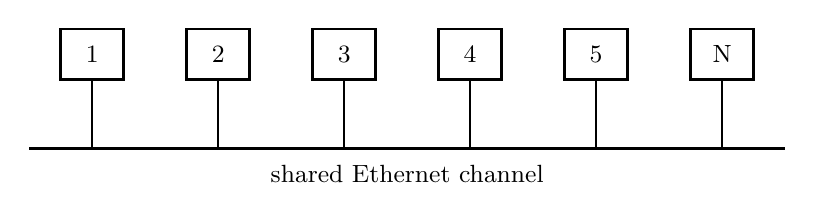
\begin{tikzpicture}[x=0.8cm,y=0.8cm]
  \draw[line width=1.1pt] (0,2.5) -- (12,2.5);
  \foreach \x/\n in {1/1,3/2,5/3,7/4,9/5,11/N} {
    \draw[line width=0.9pt] (\x,2.5) -- (\x,3.6);
    \draw[line width=0.9pt] (\x-0.5,3.6) rectangle (\x+0.5,4.4);
    \node at (\x,4.0) {\small \n};
  }
  \node at (6,2.1) {\small shared Ethernet channel};
\end{tikzpicture}
\caption{A Simple Ethernet Network}
\label{fig:ether-simple-network}
\end{figure}

Ethernet communication behavior is implemented by controller hardware (and
microcode) together with station software; exact partitioning depends on the
implementation. In general deployments, stations may be computers,
workstations, file servers, printers, and other devices. For this model,
stations are assumed identical.

Ethernet supports up to 1024 stations and a total cable length of 2.5 km in a
non-rooted tree interconnection, with repeaters for long segments. Data is
transmitted serially at 10 Mbps. Ethernet is specified in detail in
[DEC et al 1982], with a close ANSI/IEEE counterpart in 802.3.

\subsection*{Data format}

Data is transmitted in frames containing preamble, header, data, and CRC.

\begin{figure}[ht]
\centering
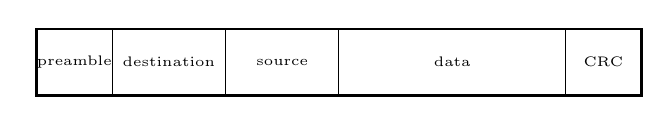
\begin{tikzpicture}[x=0.12cm,y=0.7cm]
  \draw[line width=1pt] (0,0) rectangle (64,1.2);
  \draw (8,0) -- (8,1.2); \draw (20,0) -- (20,1.2);
  \draw (32,0) -- (32,1.2); \draw (56,0) -- (56,1.2);
  \node at (4,0.6) {\tiny preamble};
  \node at (14,0.6) {\tiny destination};
  \node at (26,0.6) {\tiny source};
  \node at (44,0.6) {\tiny data};
  \node at (60,0.6) {\tiny CRC};
\end{tikzpicture}
\caption{Ethernet Frame Format}
\label{fig:ether-frame-format}
\end{figure}

The data field length is 46--1500 bytes. Shorter messages are padded to the
minimum. Header fields carry destination/source addresses and data length
(excluding padding). The CRC supports error checking at the receiver.

Before frame data, a station sends a 64-bit synchronization preamble. With
$L$ as data-field length in bytes, nominal frame transmission time is:

\begin{equation}
t_f = 20.8 + 0.8L \quad \text{microseconds}
\label{eq:ether-tf}
\end{equation}

Hence the minimum frame time (at $L=46$) is 57.6 microseconds.

\subsection*{Channel access protocol}

Ethernet uses Carrier Sense Multiple Access with Collision Detection
(CSMA/CD). A station with data to send senses the channel; if idle, it starts
transmission. There is an inter-frame gap between sensing idle and transmission
start to ensure receiving stations complete end-of-frame processing before a
new transmission begins.

During transmission, the sender continues sensing the channel. If another
station starts in the collision window, a collision occurs. A station that
detects collision aborts frame data transmission, sends a jam sequence so all
stations recognize the collision, and schedules a retransmission after a random
backoff delay.

\begin{figure}[ht]
\centering
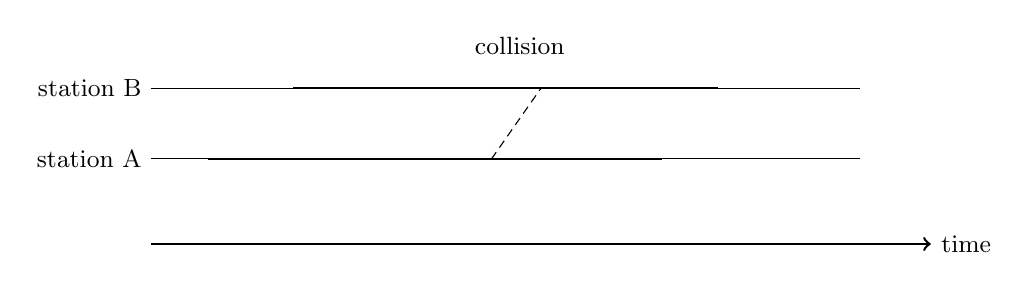
\begin{tikzpicture}[x=0.9cm,y=0.9cm]
  \draw[->,line width=0.9pt] (0,0) -- (11,0) node[right]{\small time};
  \draw (0,1.2) node[left]{\small station A} -- (10,1.2);
  \draw (0,2.2) node[left]{\small station B} -- (10,2.2);
  \draw[line width=1pt] (0.8,1.2) -- (4.8,1.2);
  \draw[line width=1pt] (2.0,2.2) -- (5.5,2.2);
  \draw[densely dashed] (4.8,1.2) -- (5.5,2.2);
  \node at (5.2,2.8) {\small collision};
  \draw[line width=0.9pt] (5.5,2.2) -- (8.0,2.2);
  \draw[line width=0.9pt] (4.8,1.2) -- (7.2,1.2);
\end{tikzpicture}
\caption{Colliding Transmissions in Ethernet}
\label{fig:ether-collision-timing}
\end{figure}

Let $\tau$ be end-to-end propagation delay and $T_{\text{jam}}$ jam time. In the
worst case, colliding stations each transmit for approximately
$2\tau + T_{\text{jam}}$ before backing off. A station that has transmitted for
$2\tau$ without collision has effectively acquired the channel for successful
completion.

With Ethernet's maximum round-trip propagation of 45 bit-times,
$\tau_{\max}=22.5\,\mu s$. With maximum jam length 48 bit-times,
$T_{\text{jam}}=4.8\,\mu s$. Thus a collision fragment can be up to 498 bit-times
($49.8\,\mu s$), which motivates the minimum valid frame size (excluding
preamble) of 64 bytes.

\paragraph{Slot time.}
The slot time $T_{\text{slot}}$ is specified as 512 bit-times ($51.2\,\mu s$).
It is the backoff rescheduling quantum. It must exceed both acquisition and
collision-fragment timing requirements while remaining small enough to avoid
unnecessary latency inflation.

\paragraph{Backoff algorithm.}
Ethernet uses truncated binary exponential backoff:
\begin{enumerate}
\item increment retransmission attempt count $n$;
\item if $n>16$, report transmission error;
\item set $k=\min(n,10)$;
\item draw random integer $r \in [0,2^k-1]$;
\item backoff delay is $r$ slot-times.
\end{enumerate}
So attempt 1 backs off 0--1 slots; attempt 2, 0--3; \ldots; attempts 10--16,
0--1023 slots.

\section{Performance Parameters and Measures}
\label{sec:ether-metrics}

The model focuses on throughput and mean frame delay as functions of offered
load, station count, inter-transmission intervals, and mean frame length.

Let $S$ denote network throughput in the common utilization-based form (fraction
of channel use carrying successful frame data). Let $T_d$ be mean frame delay
from first transmission attempt to successful completion, including queueing,
collision recovery, backoff, and transfer time.

With $T_f$ as mean no-contention frame transmission time, normalized delay is:

\begin{equation}
D = T_d / T_f
\label{eq:ether-D}
\end{equation}

For closed-system interpretation with $N$ identical stations and mean
inter-transmission interval $T_i$ (post-completion to next attempt):

\begin{equation}
G = \frac{N T_f}{T_i + T_f}
\label{eq:ether-G-closed}
\end{equation}

For open-system interpretation with external arrival rate $\lambda$:

\begin{equation}
G = \lambda T_f
\label{eq:ether-G-open}
\end{equation}

A key Ethernet parameter is

\begin{equation}
\alpha = \tau/T_f
\label{eq:ether-alpha}
\end{equation}

For fixed offered load, larger $\alpha$ (shorter frames relative to
propagation) implies more collision overhead and lower throughput.

\section{Lam's Model}
\label{sec:ether-lam}

Lam [1980] gives an analytic upper bound on CSMA/CD throughput:

\begin{equation}
S_{\max} = \left[1 + \alpha(1 + 2e)\right]^{-1}
\label{eq:ether-smax}
\end{equation}

\begin{figure}[ht]
\centering
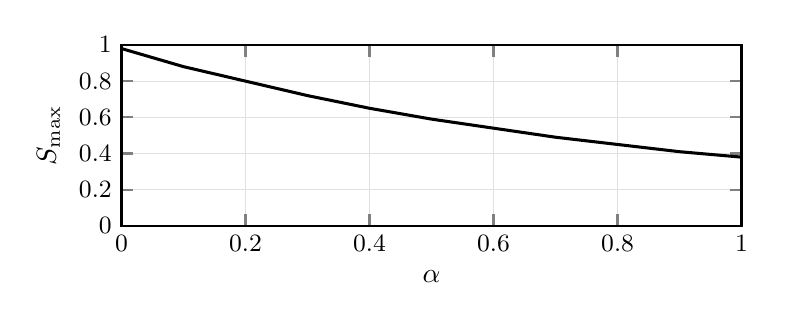
\begin{tikzpicture}
\begin{axis}[
  width=0.78\textwidth,height=0.32\textwidth,
  xmin=0,xmax=1,ymin=0,ymax=1,
  xlabel={$\alpha$},ylabel={$S_{\max}$},
  axis line style={line width=0.9pt},tick style={line width=0.8pt},
  ticklabel style={font=\small},grid=major,major grid style={draw=black!12}
]
\addplot[line width=1.1pt] table[row sep=\\]{
0.00 0.98\\ 0.05 0.93\\ 0.10 0.88\\ 0.20 0.80\\ 0.30 0.72\\
0.40 0.65\\ 0.50 0.59\\ 0.60 0.54\\ 0.70 0.49\\ 0.80 0.45\\ 0.90 0.41\\ 1.00 0.38\\
};
\end{axis}
\end{tikzpicture}
\caption{Maximum Network Throughput as a Function of $\alpha$}
\label{fig:ether-smax}
\end{figure}

Lam also provides a closed-form expression for $T_d$ in terms of
$\tau,\lambda,T_f$, moments of frame-time distribution, and Laplace transform
$B^*(\cdot)$. For constant frame lengths:
\begin{equation}
T_{f2}=T_f^2
\label{eq:ether-tf2-const}
\end{equation}
\begin{equation}
B^*(\lambda)=e^{-\lambda T_f}
\label{eq:ether-bstar-const}
\end{equation}
For exponentially distributed frame lengths:
\begin{equation}
T_{f2}=2T_f^2
\label{eq:ether-tf2-exp}
\end{equation}
\begin{equation}
B^*(\lambda)=\frac{1}{1+\lambda T_f}
\label{eq:ether-bstar-exp}
\end{equation}

The chapter includes C code for computing Lam delay (Figure 6.5).

\begin{figure}[ht]
\centering
\begin{minipage}{0.86\textwidth}
\begin{verbatim}
real lam_delay(real alpha, real rho)
{
  /* Lam approximation for non-persistent CSMA/CD */
  real a2 = alpha * alpha;
  real num = 1.0 + alpha * (1.0 + 4.5*alpha);
  real den = 2.0 * (1.0 - rho);
  real coll = rho * (1.0 + 2.0*alpha + a2) / (1.0 - rho);
  return num/den + coll;
}
\end{verbatim}
\end{minipage}
\caption{Function to Compute Lam's Mean Frame Delay}
\label{fig:ether-lam-c}
\end{figure}

\section{The \texttt{ether} Simulation Model}
\label{sec:ether-model}

In \texttt{ether}, the network is represented as a closed system with one shared
server (channel) and a station pool as request sources. Channel state is tracked
by simple variables; stations are modeled as tokens generating requests at
random (exponentially distributed inter-request intervals), contending for
channel access, and scheduling the next request after successful completion.

A central modeling issue is propagation delay. For a macroscopic model with
indistinguishable stations, timing is represented probabilistically rather than
by exact geometric station coordinates.

Assume $N$ stations equally spaced; let $d=|i-j|$ be unit distance between the
most recent channel owner $i$ and requesting station $j$. Then:

\begin{equation}
\Pr[x=d]=\frac{2(N-d)}{N(N-1)}, \quad 1\le d \le N-1
\label{eq:ether-dist-pmf}
\end{equation}

\begin{equation}
\Pr[x \le d]=\sum_{k=1}^{d}\frac{2(N-k)}{N(N-1)}
\label{eq:ether-dist-cdf-sum}
\end{equation}

\begin{equation}
\Pr[x \le d]=\frac{2Nd-d(d+1)}{N(N-1)}
\label{eq:ether-dist-cdf}
\end{equation}

For large $N$ this is approximated by:
\begin{equation}
\Pr[x \le d] \approx 1-\left(1-\frac{d}{N}\right)^2
\label{eq:ether-dist-cdf-approx}
\end{equation}

For convenience, the inter-station distance distribution is treated as
continuous, giving the random-distance generator

\begin{equation}
d = N\left[1-r^{1/2}\right]
\label{eq:ether-rand-distance}
\end{equation}

where $r$ is uniform on $[0,1]$. Since propagation delay per unit distance is
approximately $\tau/N$ for large $N$, a sample propagation delay between the
requesting station and the station last reserving/releasing the channel is

\begin{equation}
d_t = \tau\left[1-r^{1/2}\right]
\label{eq:ether-rand-delay}
\end{equation}

\subsection*{Modeling request arrivals}

With identical stations and exponential inactive intervals, request arrivals can
be modeled with a single next-arrival event instead of one outstanding event per
station.

At a given instant, let $n$ be the number of inactive stations and $T_i$ the
mean inactive interval per station. For one station, remaining inactive time
$y$ has

\begin{equation}
\Pr[y<t] = 1-e^{-t/T_i}
\label{eq:ether-y-cdf}
\end{equation}

If $x=\min(y_1,\ldots,y_n)$, then

\begin{equation}
\Pr[x<t] = 1-\{1-\Pr[y<t]\}^{n}
\label{eq:ether-min-cdf}
\end{equation}

which simplifies to

\begin{equation}
\Pr[x<t] = 1-e^{-nt/T_i}
\label{eq:ether-next-arrival-cdf}
\end{equation}

So the time to next request from the inactive pool is exponential with mean
$T_i/n$. This supports an efficient algorithm with exactly one queued
arrival event regardless of $N$.

\subsection*{Event routines}

The model uses six events (Figure~6.6): transmission arrival, deference check,
transmission start, transmission end, backoff initialization, and channel
deassert/release.

\begin{figure}[ht]
\centering
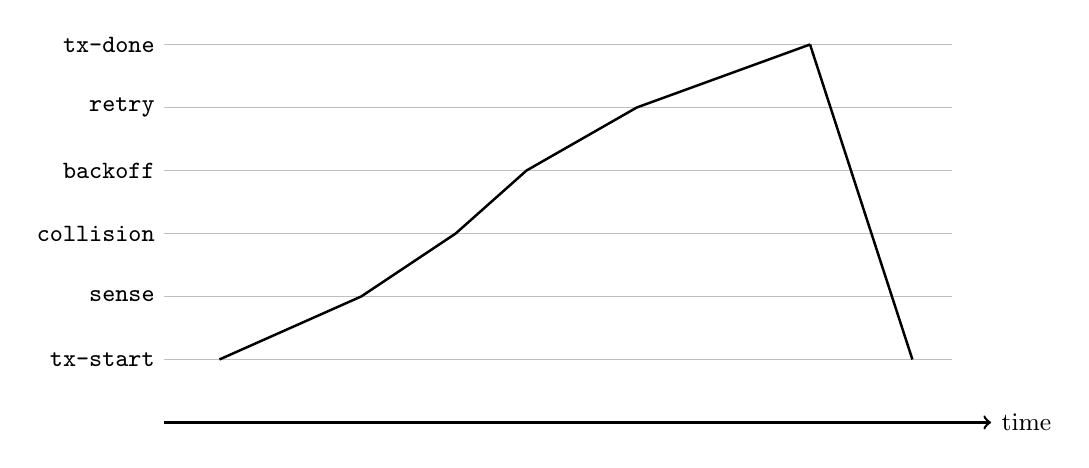
\begin{tikzpicture}[x=1cm,y=0.8cm]
  \draw[->,line width=0.9pt] (0,0) -- (10.5,0) node[right]{\small time};
  \node[left] at (0,1) {\small \texttt{tx-start}};
  \node[left] at (0,2) {\small \texttt{sense}};
  \node[left] at (0,3) {\small \texttt{collision}};
  \node[left] at (0,4) {\small \texttt{backoff}};
  \node[left] at (0,5) {\small \texttt{retry}};
  \node[left] at (0,6) {\small \texttt{tx-done}};
  \foreach \y in {1,2,3,4,5,6} {\draw[black!25] (0,\y) -- (10,\y);}
  \draw[line width=0.9pt] (0.7,1) -- (2.5,2) -- (3.7,3) -- (4.6,4) -- (6.0,5) -- (8.2,6);
  \draw[line width=0.9pt] (8.2,6) -- (9.5,1);
\end{tikzpicture}
\caption{\texttt{ether} Simulation Model Events}
\label{fig:ether-events}
\end{figure}

\textbf{TransmitFrame:} initializes attempt/backoff counters, records request
arrival time for delay measurement, schedules deference processing, decrements
inactive-station count, and schedules the next arrival using the single-event
arrival process.

\textbf{Defer:} evaluates whether a requester senses channel busy or idle,
accounting for propagation delay and inter-frame gap timing. Channel state is
tracked by status variable plus timestamps for last busy/idle transitions.

\begin{figure}[ht]
\centering
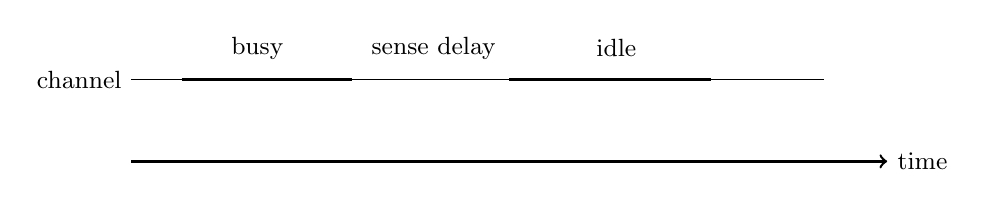
\begin{tikzpicture}[x=0.8cm,y=0.8cm]
  \draw[->,line width=0.9pt] (0,0) -- (12,0) node[right]{\small time};
  \draw (0,1.3) node[left]{\small channel} -- (11,1.3);
  \draw[line width=0.9pt] (0.8,1.3) -- (3.5,1.3);
  \draw[densely dotted] (3.5,1.3) -- (6.0,1.3);
  \draw[line width=0.9pt] (6.0,1.3) -- (9.2,1.3);
  \node at (2.0,1.8) {\small busy};
  \node at (4.8,1.8) {\small sense delay};
  \node at (7.7,1.8) {\small idle};
\end{tikzpicture}
\caption{Channel State Sensing Timing}
\label{fig:ether-sensing-timing}
\end{figure}

If busy is sensed, request is placed on defer-wait list. If idle is sensed,
remaining deference time is computed and StartTransmit is scheduled.

\begin{figure}[ht]
\centering
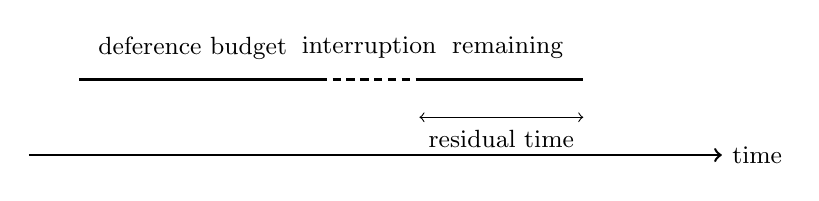
\begin{tikzpicture}[x=0.8cm,y=0.8cm]
  \draw[->,line width=0.9pt] (0,0) -- (11,0) node[right]{\small time};
  \draw[line width=0.9pt] (0.8,1.2) -- (4.6,1.2);
  \draw[densely dashed,line width=0.8pt] (4.6,1.2) -- (6.2,1.2);
  \draw[line width=0.9pt] (6.2,1.2) -- (8.8,1.2);
  \node at (2.6,1.7) {\small deference budget};
  \node at (5.4,1.7) {\small interruption};
  \node at (7.6,1.7) {\small remaining};
  \draw[<->] (6.2,0.6) -- (8.8,0.6);
  \node at (7.5,0.25) {\small residual time};
\end{tikzpicture}
\caption{Remaining Deference Time Computation}
\label{fig:ether-defer-time}
\end{figure}

\textbf{StartTransmit:} if channel is idle, reserves channel and schedules
successful completion candidate. If busy, collision is inferred: colliders are
scheduled into backoff processing and current successful-completion event may be
canceled for first detected collision in the window.

\textbf{EndTransmit:} accumulates delay statistics for successful frame,
schedules channel deassert/release, increments inactive count, and reschedules
single next-arrival event.

\textbf{InitBackoff:} applies truncated binary exponential backoff. Requests
with attempts $>16$ are dropped and source is returned to inactive pool;
otherwise requester either re-enters deference immediately (0 slots) or is
scheduled after nonzero backoff.

\textbf{Deassert:} transitions channel to idle and reactivates deferred
requests by scheduling StartTransmit after propagation plus inter-frame gap.

\section{The \texttt{ether} Simulation Program}
\label{sec:ether-program}

Figure~6.9 contains a smpl implementation of \texttt{ether}. Parameters are
defined via macros and globals (e.g., propagation delay, inter-frame gap, slot
time, jam time, station count, offered load, and $\alpha$), and event routines
directly implement the six-event logic above.

\begin{figure}[ht]
\centering
\begin{minipage}{0.86\textwidth}
\begin{verbatim}
/* ether: simplified event-driven CSMA/CD model */
main() {
  init_model();
  while (time() < TMAX) {
    cause(&ev, &src);
    switch(ev) {
      case GEN:   gen_frame(src); break;
      case SENSE: sense_channel(src); break;
      case START: start_tx(src); break;
      case COLL:  collision(src); break;
      case END:   end_tx(src); break;
      case RETRY: retry_tx(src); break;
    }
  }
  report_stats();
}
\end{verbatim}
\end{minipage}
\caption{The \texttt{ether} Simulation Program}
\label{fig:ether-program}
\end{figure}

The program estimates throughput $S$ and normalized delay $D$ as functions of
$\alpha$ and $G$. During initialization, mean frame transmission time $T_f$ and
mean inactive time $T_i$ are computed from
(\ref{eq:ether-G-closed}) and (\ref{eq:ether-alpha}). Requests are represented
with descriptor records linked through available/defer lists.

\section{\texttt{ether} Verification and Validation}
\label{sec:ether-verify-validate}

The model is checked by comparison to both Lam-model results and measured
Ethernet data.

\paragraph{Comparison with Lam-model results.}
Runs were made across $\alpha$ values (roughly 0.01--0.25) and offered loads
$G$ increasing toward saturation. For each fixed $\alpha$, throughput and delay
curves were generated and $S_{\max}$ estimated near the high-delay knee.

For smaller $\alpha$ values, simulated $S_{\max}$ tracks Lam's bound closely.
At larger $\alpha$, differences grow, largely due to model-assumption mismatch
(collision interval treatment and open-vs-closed modeling effects near
saturation).

\begin{figure}[ht]
\centering
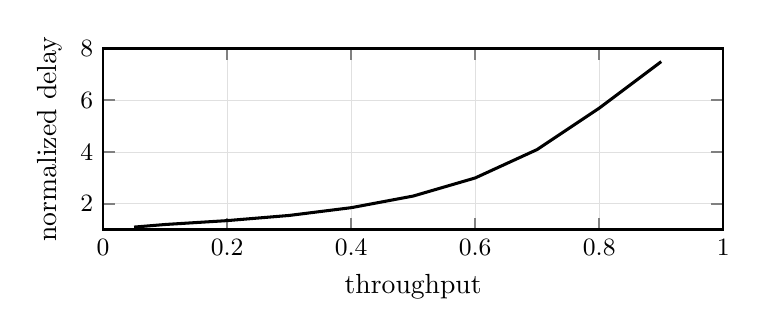
\begin{tikzpicture}
\begin{axis}[
  width=0.78\textwidth,height=0.32\textwidth,
  xmin=0,xmax=1,ymin=1,ymax=8,
  xlabel={throughput},ylabel={normalized delay},
  axis line style={line width=0.9pt},tick style={line width=0.8pt},
  ticklabel style={font=\small},grid=major,major grid style={draw=black!12}
]
\addplot[line width=1.1pt] table[row sep=\\]{
0.05 1.1\\ 0.10 1.2\\ 0.20 1.35\\ 0.30 1.55\\ 0.40 1.85\\
0.50 2.3\\ 0.60 3.0\\ 0.70 4.1\\ 0.80 5.7\\ 0.90 7.5\\
};
\end{axis}
\end{tikzpicture}
\caption{Normalized Delay versus Throughput at $\alpha=0.05$}
\label{fig:ether-delay-vs-throughput}
\end{figure}

\paragraph{Comparison with measurement data.}
To align with reported measurements (Gonsalves), simulation settings are
adjusted (notably smaller $N$, different $\tau$, constant frame lengths, and
uniform inactive intervals). Throughput definitions are also aligned: measured
throughput may be based on data bytes only, while simulation throughput is often
based on total frame time.

If $\alpha'$ is based on frame length excluding preamble and $\alpha$ includes
preamble, the relationship used is

\begin{equation}
\alpha = \alpha' \left(1 + \frac{8}{L'}\right)
\label{eq:ether-alpha-prime}
\end{equation}

Representative throughput comparison:

\begin{table}[ht]
\centering
\begin{tabular}{lccc}
\toprule
Frame bytes & $\alpha'$ & Gonsalves $S'$ & \texttt{ether} $S'$ \\
\midrule
64   & .280 & .26 & .28 \\
200  & .092 & .60 & .57 \\
512  & .026 & .72 & .72 \\
1500 & .012 & .85 & .83 \\
\bottomrule
\end{tabular}
\caption{Measurement and Simulation Throughput Results}
\label{tab:ether-measurement-compare}
\end{table}

\section{Applications and Extensions}
\label{sec:ether-extensions}

\texttt{ether} supports experimentation with protocol and collision-recovery
variants. Common extensions include:
\begin{itemize}
\item alternate backoff schemes,
\item load-adaptive access controls,
\item priority-aware or mixed-traffic policies,
\item variable frame-length distributions.
\end{itemize}

Variable frame lengths are important for realism (short control frames mixed
with long data frames). One practical variant is a truncated exponential frame
time model honoring Ethernet minimum/maximum frame constraints.

\subsection*{Generating variates from a truncated exponential}

For exponential variable $t$ with parameter $u$:

\begin{equation}
E[t] = \int_0^\infty t\,u e^{-ut}\,dt
\label{eq:ether-trunc-mean}
\end{equation}

Splitting at $t_{\min}$:

\begin{equation}
E[t] = \int_0^{t_{\min}} t\,u e^{-ut}\,dt + \int_{t_{\min}}^\infty t\,u e^{-ut}\,dt
\label{eq:ether-trunc-split}
\end{equation}

Replacing samples below $t_{\min}$ by $t_{\min}$ contributes

\begin{equation}
w = t_{\min}\Pr[t < t_{\min}] = t_{\min}\left(1-e^{-u t_{\min}}\right)
\label{eq:ether-trunc-w}
\end{equation}

and yields a target mean form

\begin{equation}
T_f = t_{\min}\left(1-e^{-u t_{\min}}\right) + \int_{t_{\min}}^\infty t\,u e^{-ut}\,dt
\label{eq:ether-trunc-tf}
\end{equation}

which simplifies to

\begin{equation}
T_f = t_{\min} + u^{-1}e^{-u t_{\min}}
\label{eq:ether-trunc-simplified}
\end{equation}

Since $u$ is implicit, Newton iteration is used in practice (book Eq.\ 6.25).

\section{Summary}
\label{sec:ether-summary}

This chapter develops a compact macroscopic Ethernet model using analytic
submodels to reduce detail while preserving key contention behavior. It is not
a full hybrid model in the strict sense, but it demonstrates how probabilistic
substructure can simplify event simulation and still support verification and
validation against analytic bounds and measured data.

\section{A Token Ring Modeling Project}
\label{sec:token-ring-project}

The project asks for a token-ring simulation model to study effects of ring
configuration and workload parameters.

\begin{figure}[ht]
\centering
\begin{tikzpicture}[x=1cm,y=1cm]
  \draw[line width=1pt] (0,0) circle (2.4);
  \foreach \a/\n in {90/1,18/2,-54/3,-126/4,162/N} {
    \node[draw,rectangle,minimum width=0.9cm,minimum height=0.6cm] at (\a:2.4) {\small \n};
  }
  \draw[-{Stealth[length=3mm]},line width=0.9pt] (30:2.4) arc[start angle=30,end angle=-20,radius=2.4];
  \node at (0,-3.0) {\small token circulates in ring direction};
\end{tikzpicture}
\caption{A Token Ring Network}
\label{fig:token-ring-network}
\end{figure}

Token and frame formats:

\begin{figure}[ht]
\centering
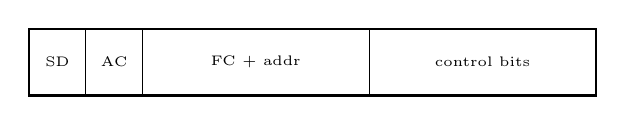
\begin{tikzpicture}[x=0.18cm,y=0.7cm]
  \draw[line width=1pt] (0,0) rectangle (40,1.2);
  \draw (4,0)--(4,1.2); \draw (8,0)--(8,1.2); \draw (24,0)--(24,1.2);
  \node at (2,0.6) {\tiny SD};
  \node at (6,0.6) {\tiny AC};
  \node at (16,0.6) {\tiny FC + addr};
  \node at (32,0.6) {\tiny control bits};
\end{tikzpicture}
\caption{Token Format}
\label{fig:token-format}
\end{figure}

\begin{figure}[ht]
\centering
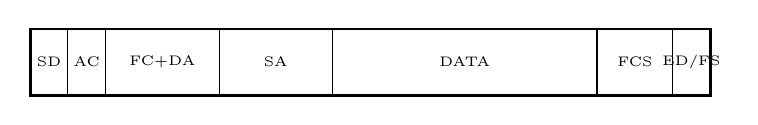
\begin{tikzpicture}[x=0.12cm,y=0.7cm]
  \draw[line width=1pt] (0,0) rectangle (72,1.2);
  \foreach \x in {4,8,20,32,60,68} {\draw (\x,0)--(\x,1.2);} 
  \node at (2,0.6) {\tiny SD};
  \node at (6,0.6) {\tiny AC};
  \node at (14,0.6) {\tiny FC+DA};
  \node at (26,0.6) {\tiny SA};
  \node at (46,0.6) {\tiny DATA};
  \node at (64,0.6) {\tiny FCS};
  \node at (70,0.6) {\tiny ED/FS};
\end{tikzpicture}
\caption{Token Ring Frame Format}
\label{fig:token-frame-format}
\end{figure}

Core network parameters:
\begin{equation}
\tau = 5K + \frac{BN}{R}
\label{eq:token-latency}
\end{equation}
\begin{equation}
T_f = \frac{L}{R}
\label{eq:token-tf}
\end{equation}
\begin{equation}
\alpha = \frac{\tau}{T_f}
\label{eq:token-alpha}
\end{equation}
\begin{equation}
S = N\lambda T_f
\label{eq:token-throughput}
\end{equation}

The chapter also provides a closed-form mean-delay expression (Eq.\ 6.31) for a
symmetric token-ring case under simplifying assumptions (Poisson arrivals,
constant frame length, uniform station spacing, and $\alpha<1$), and then asks
for simulation-based verification and exploration.

Project tasks include:
\begin{enumerate}
\item verify model behavior against Eq.\ 6.31 for baseline parameters;
\item study ring-latency impact by changing cable length and station overhead;
\item study asymmetric-arrival effects (small high-load subset of stations);
\item extend to a file-server ring workload and estimate read response-time
  components (network vs disk).
\end{enumerate}
